

В работе был рассмотрен ?вопрос проектировки? беспилотного летательного аппарата (БПЛА), предназаченного для длительного ($\approx24$~часа без дозаправки) барражирования в целях мониторинга и разведки (ограничения по режимам полета представлены на Рис.\ref{fig:ModeOfFlight}). В связи с этим к БПЛА были предъявлены высокие требования по малозаметности и аэродинамическому качеству. 


За основу была взята разработанная в ЦАГИ модель БПЛА, хорошо отвечающая требованиям аэродинамического качества и малозаметности. Вид фюзеляжа выбранной модели показан на Рис.\ref{fig:BPLA_TSAGI}.
 

%Возможно, вставить пункт с геометрическими ограничениями
  
  



\begin{figure}[ht]
\centering
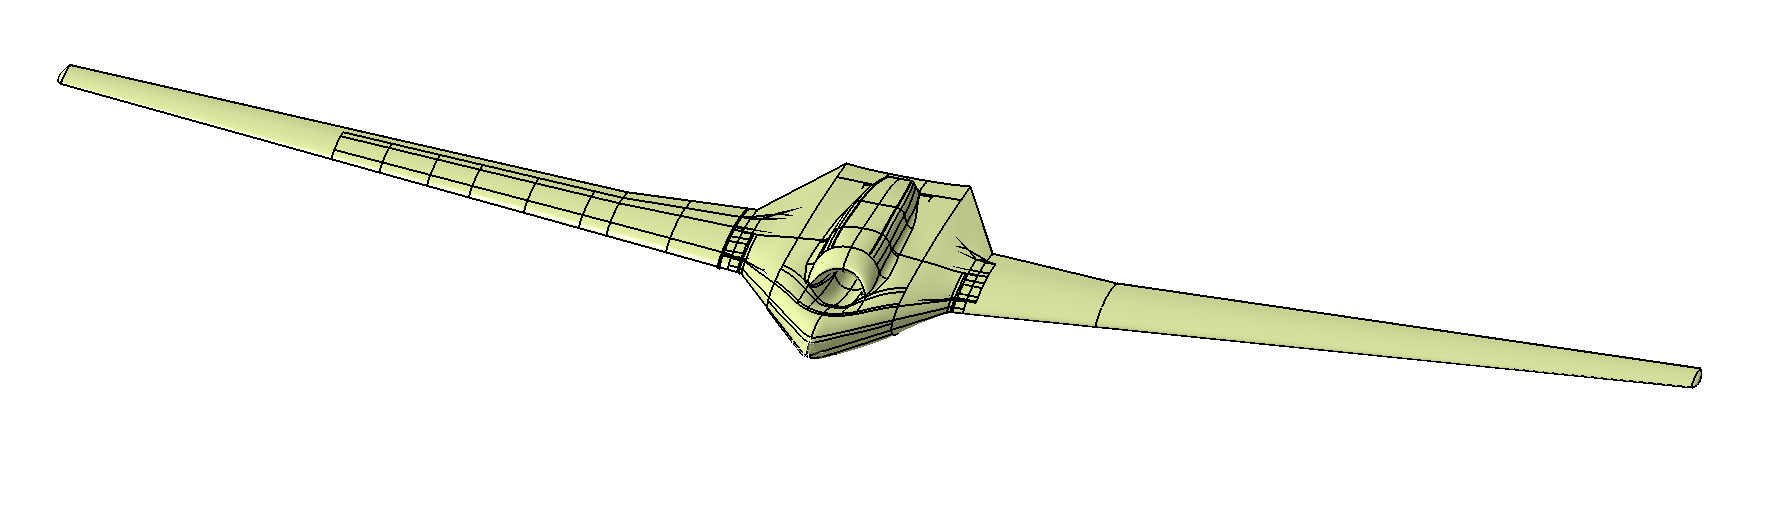
\includegraphics[width=1\textwidth]{BPS_Catia_Full}
\caption{Вид модели БПЛА-ЦАГИ}
\label{fig:BPLA_TSAGI}
\end{figure}

Данная модель выполнена по схеме ``бесхвостка'' с крылом большого удлинения, интегрированным с фюзеляжем. 

Для интеграции двигателя с воздухозаборником в конструкцию данной модели в конструкции используется изогнутый центроплан. Использование такой формы центроплана сопряжено с возможным возникновением проблем обеспечения прочности в связи с большими изгибающими моментами в нём. 

Использование такого центроплана может существенно ухудшить компоновку и весовую эффективность БПЛА по сравнению с использованием прямого центроплана. Исследований центропланов такой формы ранее не проводилось. В данной работе проведен анализ возможных ухудшений весовой эффективности. 
 
%очевидно, что волнообразный центроплан может иметь напряжные вопросы с обеспечением прочности, т.к. такие центропланы в такой размерности не использовались, довольно нагружены. Сказать про компоновку, нарисовать её (общие вещи).

%с самого начала пишем, какие проблемы. Так сделали, такая компоновка, но у неё такие-то проблемы след волнообразный центроплан

%дальше: это может существенно ухудшить компоновку и весовую эффективность по сравнению с прямым центропланом. Цель работы - оценить возможные ухудшения. 

% и уже для того, чтобы оценить: следующий параграф 

Для оценки возможных ухудшений весовой эффективности и компоновки была поставлена задача построения расчетной модели данного БПЛА и прочностного анализа созданной модели. 
При построении модели необходимо было учесть ее дальнейшую модификацию, позволяющую варьировать форму внешних аэродинамических обводов. В бакалаврской работе форма внешних аэродинамических обводов постоянны. Также постоянными считаются нагрузки на конструкцию (см.Раздел \ref{sec:externalLoads}). 

%В бакалаврской работе будем рассматривать только те обводы, которые есть в этой модели. И целью работы будет оценка потерь из-за такого центроплана (в прочности)

 
  
  

%Не забыть про то, что мы также хотим менять аэродинамику
%Требования: БПЛА, полет на таких-то высотах, столько-то. Весовая сводка такая-то, максимальные перегрузки, коэффициент запаса, аэродинамика. Ограничения - малозаметность, вес, пожаробезопасность отсека двигателя. 
%

